

\chapter {Debugging features}
\label{sec:Debugging}

During the development of the extensions here portraited, there were a variety of problems for the proper integration and configuration of the stack. It was deemed convenient to add some changes to the version of the ToolChain that was used during the development to easen the pinpointing of errors.

\section {FreeRTOS Stack Overflow Check}
\label{sec:FreeRTOS Stack Overflow}

Each task spawned by FreeRTOS has a stack assigned to it with a size determined by one of the arguments in the task creation function.

\begin{lstlisting}
  void ttc_task_create(
  void TaskFunction(void*),   // function to start as thread
  const signed char* TaskName,// thread name (just for debugging)
  u16_t StackSize,            // stack size
  void* Argument,             // passed as argument to the task
  u8_t Priority,              // task priority (higher values mean more process time)
  void* Handle                // can return a handle to created task
  );
\end{lstlisting}

When the memory consumed by the task stack exceeds this ``StackSize`` parameter, a Stack overflow is produced, leading to instability.

FreeRTOS offers two methods for detecting a Stack Overflow, and even though they are only available on architectures where the memory map is not segmented, this is the case for the stm32 cortex family.

\begin{itemize}
\item It is likely that the stack will reach its greatest (deepest) value after the RTOS kernel has swapped the task out of the Running state because this is when the stack will contain the task context. At this point the RTOS kernel can check that the processor stack pointer remains within the valid stack space. The stack overflow hook function is called if the stack pointer contain a value that is outside of the valid stack range.
  This method is quick but not guaranteed to catch all stack overflows.

\item When a task is first created its stack is filled with a known value. When swapping a task out of the Running state the RTOS kernel can check the last 16 bytes within the valid stack range to ensure that these known values have not been overwritten by the task or interrupt activity. The stack overflow hook function is called should any of these 16 bytes not remain at their initial value.
  This method is less efficient than method one, but still fairly fast. It is very likely to catch stack overflows but is still not guaranteed to catch all overflows.

\end{itemize}

\section {Fault Stack Check}

\subsection { Registers from the fault stack  }

\begin{lstlisting}
  // If no stack was passed, retrieve it
  if( fault_stack == 0 ) {
    __asm__ volatile
    ( // Assembly code to retrieve register information
    " TST LR, #4    \n" // Substract 4 from LR (will obtain the faulty instruction)
    " ITE EQ        \n" // If EQ
    " MRSEQ R0, MSP \n" // Then.. move Main Stack    to R0
    " MRSNE R0, PSP \n" // Else.. move Process Stack to R0
    " B FaultStack_Check " // jump back to function (with the stack as parameter)
    );
  }

  u32_t R0  = fault_stack[0]; // R0-R12: General-purpose
  u32_t R1  = fault_stack[1];
  u32_t R2  = fault_stack[2];
  u32_t R3  = fault_stack[3];
  u32_t R12 = fault_stack[4];
  u32_t LR  = fault_stack[5]; // Link Register   (R14)
  u32_t PC  = fault_stack[6]; // Program Counter (R15)
  u32_t PSR = fault_stack[7]; // Program Status Register
\end{lstlisting}


\subsection{Registers holding the fault status}

\begin{figure}[H]
  \begin{center}
    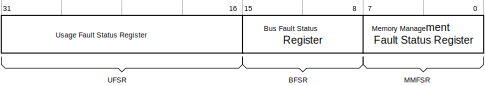
\includegraphics[width=\textwidth]{images/CFSR} \\
    \includegraphics[width=0.5\textwidth]{images/MMFSR} \\
    \includegraphics[width=0.5\textwidth]{images/BFSR} \\
    \includegraphics[width=0.5\textwidth]{images/UFSR}
  \end{center}
  \caption{Configurable Fault Status Register}
  \label{fig:CFSR}
\end{figure}

In the figure \ref{fig:CFSR} we can see the structure of the register labeled as CFSR (Configurable Fault Status Register).

This register contains varied information that can be very useful for determining the cause of a problem when a fault occurs. The relevant bits of information are determined by what kind of fault was triggered: Hard Fault, Memory Management Fault, Bus Fault, or Usage Fault.

\begin{itemize}
    \item Hard Fault - default Fault Handler triggered on unknown errors or when the appropiate handler is disabled.
    \item Memory Management Fault - triggered when attempting to access unprivileged memory
    \item Bus Fault - triggered when attempting to access an invalid or offline memory region
    \item Usage Fault - triggered on undefined instructions or some other unaligned access
\end{itemize}

To enable the respective fault handlers, the pertinents bits in the SHCSR register must be set.

\begin{lstlisting}
    // Enable BusFault, UsageFault and MemManage interrupts
    SCB->SHCSR |= (SCB_SHCSR_BUSFAULTENA_Msk | SCB_SHCSR_USGFAULTENA_Msk | SCB_SHCSR_MEMFAULTENA_Msk);
\end{lstlisting}

\newpage

\begin{lstlisting}
  struct { // Configurable Fault Status Register

    struct { // Memory Management Fault Status Register (8b)
      unsigned IACCVIOL  : 1; // =1: Instruction access violation
      unsigned DACCVIOL  : 1; // =1: Data access violation
      unsigned reserved2 : 1;
      unsigned UNMSTKERR : 1; // =1: MemManage fault on unstacking for a return from exception
      unsigned MSTKERR   : 1; // =1: MemManage fault on stacking for exception entry
      unsigned reserved1 : 2;
      unsigned MMARVALID : 1; // =1: MMAR is known
    } MMFSR; // Memory Management Fault Status Register (8b)

    struct { // Bus Fault Status Register (8b)
      unsigned IBUSERR     : 1; // =1: Instruction bus error
      unsigned PRECISERR   : 1; // =1: Data bus error, the PC has the intruction causing the fault
      unsigned IMPRECISERR : 1; // =1: Data bus error asynchronouns, PC advanced after the error
      unsigned UNSTKERR    : 1; // =1: BusFault on unstacking for a return from exception
      unsigned STKERR      : 1; // =1: BusFault on stacking for exception entry
      unsigned reserved1   : 2;
      unsigned BFARVALID   : 1; // =1: BFAR is known
    } BFSR;  // Bus Fault Status Register (8b)

    struct { // Usage Fault Status Register (16b)
      unsigned reserved1  : 6;
      unsigned DIVBYZERO  : 1; // =1: Division by zero
      unsigned UNALIGNED  : 1; // =1: Unaligned memory access
      unsigned reserved2  : 4;
      unsigned NOCP       : 1; // =1: Attempted to use a coprocessor
      unsigned INVPC      : 1; // =1: Invalid PC load (illegal EXC_RETURN)
      unsigned INVSTATE   : 1; // =1: Illegal use of EPSR (Execution Program Status)
      unsigned UNDEFINSTR : 1; // =1: Attempted to execute an undefined instruction
    } UFSR;  // Usage Fault Status Register (16b)

  } CFSR;  // Configurable Fault Status Register
\end{lstlisting}


Some useful debugger commands:

\begin{itemize}
\item  \verb/l *PC/ \\
  Shows line executed when the interrupt was triggereda

\item  \verb/l *LR/ \\
  Shows last function call

\item  \verb/p CFSR/ \\
  Shows struct with information about the fault
\item  \verb/p (CFSR.BFSR.BFARVALID)?BFAR:0/ \\
  Location that generated a Bus Fault (0 if no BusFault)
\item  \verb/p (CFSR.MMSR.MMARVALID)?MMFAR:0/ \\
  Location that generated a MemManage Fault (0 if no MMFault)
\end{itemize}

The most common error is Imprecise Bus Fault (CFSR.BFSR.IMPRECISERR = 1) meaning that there was an attempt to write in an invalid address, and since this access was asynchronous the PC might be 1 or more lines ahead (so the actual faulty instruction might be a little before). Also, since the PC is usually in some binary code without source, LR can be useful.


